% Apuntes de clase de ejemplo, escritos en KalaScript sobre hoja cuadriculada.
% Compilar con: make apuntes
\documentclass[11pt,a4paper]{article}
% Configuración compartida por KalaScript.tex y atlas.tex.
\usepackage[T1]{fontenc}
\usepackage[utf8]{inputenc}
\usepackage{lmodern}
\usepackage{babel}
\babelprovide[main,import]{spanish}
\usepackage[a4paper,margin=22mm,headheight=16pt]{geometry}
\usepackage{microtype}
\usepackage{amsmath,amssymb}
\usepackage{graphicx,xcolor,tikz}
\usepackage{booktabs,longtable,array,tabularx}
\usepackage{enumitem,fancyvrb,fancyhdr,titlesec}
\usepackage{xurl}
\usepackage[unicode,hidelinks]{hyperref}

\definecolor{KalaTinta}{HTML}{263B35}
\definecolor{KalaSuave}{HTML}{616C66}
\definecolor{KalaAcento}{HTML}{A75735}
\definecolor{KalaLinea}{HTML}{D7DDD3}
\definecolor{KalaPapel}{HTML}{F7F5EE}
\definecolor{KalaVerde}{HTML}{E6EBE1}
\hypersetup{pdftitle={KalaScript · Núcleo escrito},
  pdfsubject={Escritura visual, gramática y ejemplos},
  colorlinks=true,linkcolor=KalaTinta,urlcolor=KalaAcento,
  bookmarksnumbered=true}
\setlength{\parindent}{0pt}
\setlength{\parskip}{6pt plus 1pt}
\setlength{\emergencystretch}{2em}
\setlist{itemsep=3pt,topsep=5pt,leftmargin=*}
\renewcommand{\arraystretch}{1.15}
\renewcommand{\contentsname}{Contenido}
\renewcommand{\tablename}{Tabla}
\renewcommand{\figurename}{Figura}
\titleformat{\section}{\Large\sffamily\color{KalaTinta}}{\thesection}{.7em}{}
\titleformat{\subsection}{\large\sffamily\color{KalaTinta}}{\thesubsection}{.7em}{}
\titleformat{\subsubsection}{\normalsize\sffamily\bfseries\color{KalaTinta}}{\thesubsubsection}{.7em}{}
\pagestyle{fancy}
\fancyhf{}
\fancyhead[L]{\small\sffamily\color{KalaSuave}KalaScript}
\fancyhead[R]{\small\sffamily\color{KalaSuave}Núcleo escrito}
\fancyfoot[L]{\footnotesize\sffamily\color{KalaSuave}Escritura personal}
\fancyfoot[R]{\small\sffamily\thepage}
\renewcommand{\headrulewidth}{.3pt}
\renewcommand{\footrulewidth}{0pt}

% Registro único: código, nombre, familia, definición, trayectos, dibujo.
\newcommand{\KalaRegistrar}[6]{%
  \expandafter\def\csname KalaNombre#1\endcsname{#2}%
  \expandafter\def\csname KalaFamilia#1\endcsname{#3}%
  \expandafter\def\csname KalaDescripcion#1\endcsname{#4}%
  \expandafter\def\csname KalaTrayectos#1\endcsname{#5}%
  \expandafter\def\csname KalaDibujo#1\endcsname{#6}%
}
\newcommand{\KalaSimbolo}[2][9mm]{%
  \begingroup
  \ifcsname KalaDibujo#2\endcsname\else
    \PackageError{KalaScript}{Simbolo desconocido: #2}{Use un codigo del catalogo.}%
  \fi
  \pgfmathsetlengthmacro{\KalaUnidad}{#1/64}%
  \pgfmathsetlengthmacro{\KalaGrosor}{#1*2.6/64}%
  \begin{tikzpicture}[x=\KalaUnidad,y=-\KalaUnidad,
    baseline={([yshift=-.55ex]current bounding box.center)},
    draw=KalaTinta,line width=\KalaGrosor,line cap=round,line join=round]
    \path[use as bounding box] (0,0) rectangle (64,64);
    \csname KalaDibujo#2\endcsname
  \end{tikzpicture}%
  \endgroup
}
\newcommand{\KalaGrupo}[1]{%
  \tikz[baseline={([yshift=-.55ex]current bounding box.center)}]
    \node[draw=KalaSuave,line width=.35pt,rounded corners=.6pt,
      inner xsep=4pt,inner ysep=4pt]{#1};%
}
\newcommand{\KalaMat}[1]{%
  \tikz[baseline={([yshift=-.55ex]current bounding box.center)}]
    \node[draw=KalaSuave,dashed,line width=.35pt,fill=KalaPapel,
      inner xsep=4pt,inner ysep=3pt]{\ensuremath{\displaystyle #1}};%
}
\newcommand{\KalaReferencia}[1]{\KalaSimbolo{K10}\kern-.8mm\textsubscript{#1}}
\newcommand{\KalaSeparador}{\kern1.4mm\textcolor{KalaSuave}{\ensuremath{\mid}}\kern1.4mm}
\newcommand{\KalaRelacion}[2]{\KalaSimbolo{K03}\kern-.8mm\textsubscript{#1}\kern1.5mm\KalaGrupo{#2}}
\newcommand{\KalaNegacion}[1]{\KalaSimbolo{K11}\kern1mm\KalaGrupo{#1}}
\newcommand{\KalaConjuncion}[2]{\KalaSimbolo{K12}\kern1mm\KalaGrupo{#1\KalaSeparador#2}}
\newcommand{\KalaCondicional}[2]{\KalaSimbolo{K13}\kern1mm\KalaGrupo{#1\KalaSeparador#2}}
\newcommand{\KalaUniversal}[3]{\KalaSimbolo{K14}\kern1mm\ensuremath{#1\in}\,\KalaMat{#2}\kern1mm\KalaGrupo{#3}}
\newcommand{\KalaExistencia}[3]{\KalaSimbolo{K15}\kern1mm\ensuremath{#1\in}\,\KalaMat{#2}\kern1mm\KalaGrupo{#3}}
\newcommand{\KalaFuente}[2]{\KalaSimbolo{K16}\kern1mm#1\kern1mm\KalaGrupo{#2}}
\newcommand{\KalaDefinicion}[2]{\KalaSimbolo{K09}\kern1mm\ensuremath{#1}\kern1mm\KalaGrupo{#2}}
\newsavebox{\KalaCajaExpresion}
\newcommand{\KalaMostrar}[1]{%
  \begin{center}
  \sbox{\KalaCajaExpresion}{#1}%
  \ifdim\wd\KalaCajaExpresion>\linewidth
    \resizebox{\linewidth}{!}{\usebox{\KalaCajaExpresion}}%
  \else\usebox{\KalaCajaExpresion}\fi
  \end{center}%
}
\newcommand{\KalaTarjeta}[1]{%
  \begin{minipage}[t]{.235\linewidth}
  \setlength{\fboxsep}{3mm}%
  \fcolorbox{KalaLinea}{KalaPapel}{%
    \parbox[c][33mm][c]{\dimexpr\linewidth-2\fboxsep-2\fboxrule\relax}{%
      {\scriptsize\sffamily\color{KalaSuave}#1\hfill\csname KalaFamilia#1\endcsname}\par
      \centering\vspace{1mm}\KalaSimbolo[16mm]{#1}\par\vspace{1mm}
      {\small\sffamily\csname KalaNombre#1\endcsname}%
    }}%
  \end{minipage}%
}
\newcommand{\KalaCatalogoFila}[1]{%
  \KalaSimbolo[10mm]{#1}\quad\texttt{#1}&
  \textbf{\csname KalaNombre#1\endcsname}\par
  \csname KalaDescripcion#1\endcsname\par
  {\footnotesize\color{KalaSuave}\csname KalaFamilia#1\endcsname\;·\;
   \csname KalaTrayectos#1\endcsname\
   \ifnum\csname KalaTrayectos#1\endcsname=1 trayecto propuesto\else trayectos propuestos\fi.}\\[5pt]
}
% Inventario base de KalaScript, con las revisiones gráficas aceptadas.
% Coordenadas: cuadrícula 64 × 64, origen superior izquierdo.
% Editar directamente en LaTeX; no depende de SVG ni JSON.

\KalaRegistrar{K01}{Entidad}{Categoría}
  {Un objeto del dominio del que se habla; no identifica por sí solo un objeto particular.}{2}{%
  \draw (18,18) -- (18,40) .. controls (18,46) and (21.333333,49) .. (28,49) -- (44,49);
  \draw (30,15) -- (46,15) -- (46,31);
}

\KalaRegistrar{K02}{Propiedad}{Categoría}
  {Una característica atribuible a una entidad dentro de un dominio definido.}{2}{%
  \draw (16,44) .. controls (16,28) and (22,20) .. (34,20) .. controls (42,20) and (46,24.666667) .. (46,34) -- (32,34);
  \draw (32,34) -- (32,49);
}

\KalaRegistrar{K03}{Relación}{Categoría}
  {Con un índice y argumentos, aplica una relación del catálogo. El orden de los argumentos es significativo.}{2}{%
  \draw (13,42) .. controls (19,42) and (23.333333,38.333333) .. (26,31) .. controls (28.666667,23.666667) and (33,20) .. (39,20) -- (51,20);
  \draw (42,12) -- (51,20) -- (43,29);
}

\KalaRegistrar{K04}{Proceso}{Categoría}
  {Una actividad o transformación considerada en un dominio. No implica automáticamente causalidad.}{2}{%
  \draw (14,43) .. controls (14,26) and (30,26) .. (30,43) .. controls (30,58) and (47,49) .. (47,25);
  \draw (40,30) -- (47,22) -- (54,29);
}

\KalaRegistrar{K05}{Cantidad}{Categoría}
  {Una magnitud expresable mediante un valor y, cuando corresponde, una unidad.}{3}{%
  \draw (19,15) -- (19,48) -- (47,48);
  \draw (19,26) -- (36,26);
  \draw (19,37) -- (43,37);
}

\KalaRegistrar{K06}{Colección}{Categoría}
  {Una agrupación cuya naturaleza se declara: conjunto, lista u otra estructura. No impone orden ni unicidad por sí sola.}{2}{%
  \draw (24,14) .. controls (8,14) and (8,50) .. (24,50);
  \draw (34,22) -- (47,22) -- (34,42) -- (47,42);
}

\KalaRegistrar{K07}{Tiempo}{Categoría}
  {Un aspecto temporal, como instante o intervalo, con referencia temporal declarada cuando sea necesaria.}{2}{%
  \draw (17,16) .. controls (38.333333,16) and (49,21.333333) .. (49,32) .. controls (49,42.666667) and (38.333333,48) .. (17,48);
  \draw (18,25) -- (18,39) -- (29,39);
}

\KalaRegistrar{K08}{Espacio}{Categoría}
  {Un aspecto espacial cuya interpretación requiere dominio, escala o marco de referencia cuando corresponda.}{2}{%
  \draw (15,36) -- (32,15) -- (49,36) -- (32,49) -- cycle;
  % La barra termina en el centro del lado oblicuo, sin sobresalir.
  \draw (32,32) -- (45.761905,32);
}

\KalaRegistrar{K09}{Definición}{Marcador}
  {Introduce una definición nombrada. No afirma haber demostrado un resultado.}{3}{%
  \draw (14,18) -- (25,18) -- (25,46) -- (14,46);
  \draw (34,25) -- (51,25);
  \draw (34,39) -- (51,39);
}

\KalaRegistrar{K10}{Referencia}{Marcador}
  {Seguida de un índice, remite al referente definido en la leyenda del documento.}{1}{%
  \draw (17,44) -- (17,20) .. controls (17,16) and (19,14) .. (23,14) -- (41,14) -- (41,35) -- (29,35);
}

\KalaRegistrar{K11}{Negación}{Operador}
  {Niega la proposición de su grupo. No forma antónimos ni indica desconocimiento.}{2}{%
  \draw (15,19) .. controls (31,11) and (49,21) .. (49,36) .. controls (49,44) and (44.666667,48.333333) .. (36,49);
  \draw (19,50) -- (43,13);
}

\KalaRegistrar{K12}{Conjunción}{Operador}
  {Afirma conjuntamente dos proposiciones, sin afirmar un orden temporal entre ellas.}{2}{%
  \draw (14,20) -- (32,45) -- (50,20);
  \draw (32,45) -- (32,53);
}

\KalaRegistrar{K13}{Condicional}{Operador}
  {Implicación material clásica entre antecedente y consecuente. No significa causa ni ejecución.}{2}{%
  \draw (14,19) -- (32,32) -- (14,45);
  \draw (32,32) -- (50,32) -- (44,24);
}

\KalaRegistrar{K14}{Universal}{Operador}
  {Para cada elemento del dominio indicado se cumple el cuerpo agrupado.}{3}{%
  \draw (15,18) -- (15,45) .. controls (26.333333,51.666667) and (37.666667,51.666667) .. (49,45) -- (49,18);
  \draw (15,28) -- (49,28);
  \draw (32,12) -- (32,41);
}

\KalaRegistrar{K15}{Existencia}{Operador}
  {Existe al menos un elemento del dominio indicado para el que se cumple el cuerpo agrupado.}{2}{%
  \draw (15,18) -- (15,45) .. controls (26.333333,51.666667) and (37.666667,51.666667) .. (49,45) -- (49,18);
  \draw (25,28) -- (39,28);
}

\KalaRegistrar{K16}{Fuente}{Marcador}
  {Atribuye una proposición a una fuente identificada. No certifica su verdad ni cuantifica confianza.}{2}{%
  \draw (16,48) -- (16,16) -- (38,16) -- (49,27) -- (49,48) -- cycle;
  \draw (25,32) -- (39,32);
}

% Seis signos funcionales nuevos. Propuestas gráficas pendientes de prueba manual.
\KalaRegistrar{K17}{Alternativa}{Operador}
  {Disyunción inclusiva de dos proposiciones: al menos una es verdadera; pueden serlo ambas.}{2}{%
  \draw (14,18) -- (30,32) -- (14,46);
  \draw (50,18) -- (34,32) -- (50,46);
}
\KalaRegistrar{K18}{Posibilidad}{Operador}
  {Con un índice de modelo, afirma que el cuerpo se cumple en algún estado accesible. Fragmento modal proposicional.}{2}{%
  \draw (44,14) -- (20,14) .. controls (12,14) and (12,18) .. (12,26) -- (12,42) .. controls (12,50) and (16,50) .. (24,50) -- (44,50);
  \draw (32,23) -- (43,32) -- (32,41);
}
\KalaRegistrar{K19}{Pregunta}{Marcador}
  {Pregunta si la proposición agrupada es verdadera. Solo aparece en el nivel superior; no afirma el contenido.}{1}{%
  \draw (14,43) .. controls (14,16) and (45,14) .. (49,30) -- (33,40) -- (49,50);
}
\KalaRegistrar{K20}{Selección}{Constructor}
  {Construye el conjunto de elementos de un dominio que cumplen una condición. Vincula una variable en el cuerpo.}{2}{%
  \draw (14,16) -- (50,16) -- (35,34) -- (35,49);
  \draw (22,25) -- (42,25);
}
\KalaRegistrar{K21}{Secuencia}{Programa}
  {Ejecuta el primer programa y después el segundo. El segundo comienza solo si el primero termina.}{2}{%
  \draw (14,45) -- (14,32) -- (31,32) -- (31,19) -- (49,19);
  \draw (41,11) -- (49,19) -- (41,27);
}
\KalaRegistrar{K22}{Mientras}{Programa}
  {Comprueba una condición antes de cada iteración y ejecuta el cuerpo mientras sea verdadera. Puede no terminar.}{1}{%
  % Arco y barra en un solo trayecto; se elimina el segmento superpuesto.
  \draw (46,20) .. controls (20,5) and (9,33) .. (22,46) .. controls (34,58) and (54,41) .. (47,30) -- (37,30);
}

% Alias conservados para los comandos del cuaderno de comparación.
\KalaRegistrar{V06}{Colección B}{Aceptada}
  {Forma simplificada aceptada de K06. Alias gráfico de la forma habitual.}{2}{%
  \csname KalaDibujoK06\endcsname
}
\KalaRegistrar{V16}{Fuente B}{Aceptada}
  {Forma simplificada aceptada de K16. Alias gráfico de la forma habitual.}{2}{%
  \csname KalaDibujoK16\endcsname
}

% Formas anteriores, conservadas para leer y comparar documentos históricos.

\KalaRegistrar{H06}{Colección A}{Anterior}
  {Una agrupación cuya naturaleza se declara: conjunto, lista u otra estructura. No impone orden ni unicidad por sí sola.}{4}{%
  \draw (21,12) .. controls (10,12) and (13,24) .. (20,27) -- (14,32) -- (20,37) .. controls (13,40) and (10,52) .. (21,52);
  \draw (31,22) -- (46,22);
  \draw (31,32) -- (46,32);
  \draw (31,42) -- (46,42);
}

\KalaRegistrar{H16}{Fuente A}{Anterior}
  {Atribuye una proposición a una fuente identificada. No certifica su verdad ni cuantifica confianza.}{3}{%
  \draw (14,46) -- (14,19) -- (41,19) -- (41,46) -- cycle;
  \draw (22,11) -- (50,11) -- (50,37);
  \draw (22,29) -- (33,29);
}

% Construcciones escritas 0.2.0; las macros 0.1 siguen disponibles.
\newcommand{\KalaConcepto}[1]{\KalaSimbolo{K01}\kern-.8mm\textsubscript{#1}}
\newcommand{\KalaPropiedad}[1]{\KalaSimbolo{K02}\kern-.8mm\textsubscript{#1}}
\newcommand{\KalaVariable}[1]{\ensuremath{#1}}
\newcommand{\KalaColeccion}[2]{\KalaSimbolo{K06}\kern-.8mm\textsubscript{#1}\kern1mm\KalaGrupo{#2}}
\newcommand{\KalaTodo}[3]{\KalaSimbolo{K14}\kern1mm\ensuremath{#1\in}\,#2\kern1mm\KalaGrupo{#3}}
\newcommand{\KalaExiste}[3]{\KalaSimbolo{K15}\kern1mm\ensuremath{#1\in}\,#2\kern1mm\KalaGrupo{#3}}
\newcommand{\KalaAlternativa}[2]{\KalaSimbolo{K17}\kern1mm\KalaGrupo{#1\KalaSeparador#2}}
\newcommand{\KalaPosible}[2]{\KalaSimbolo{K18}\kern-.8mm\textsubscript{#1}\kern1mm\KalaGrupo{#2}}
\newcommand{\KalaPregunta}[1]{\KalaSimbolo{K19}\kern1mm\KalaGrupo{#1}}
\newcommand{\KalaSeleccion}[3]{\KalaSimbolo{K20}\kern1mm\ensuremath{#1\in}\,#2\kern1mm\KalaGrupo{#3}}
\newcommand{\KalaSecuencia}[2]{\KalaSimbolo{K21}\kern1mm\KalaGrupo{#1\KalaSeparador#2}}
\newcommand{\KalaMientras}[2]{\KalaSimbolo{K22}\kern1mm\KalaGrupo{#1\KalaSeparador#2}}
\newcommand{\KalaAsignar}[2]{\KalaSimbolo{K04}\kern-.8mm\textsubscript{1}\kern1mm\KalaGrupo{\KalaVariable{#1}\KalaSeparador\KalaMat{#2}}}
\newcommand{\KalaPosee}[2]{\KalaRelacion{8}{#1\KalaSeparador\KalaPropiedad{#2}}}
\newcommand{\KalaMiembro}[2]{\KalaRelacion{5}{#1\KalaSeparador#2}}
\newcommand{\KalaGusta}[2]{\KalaRelacion{7}{#1\KalaSeparador#2}}
\newcommand{\KalaFuenteB}[2]{\KalaSimbolo{V16}\kern1mm#1\kern1mm\KalaGrupo{#2}}
\newcommand{\KalaColeccionB}[2]{\KalaSimbolo{V06}\kern-.8mm\textsubscript{#1}\kern1mm\KalaGrupo{#2}}
\newcommand{\KalaFuenteAnterior}[2]{\KalaSimbolo{H16}\kern1mm#1\kern1mm\KalaGrupo{#2}}
\newcommand{\KalaColeccionAnterior}[2]{\KalaSimbolo{H06}\kern-.8mm\textsubscript{#1}\kern1mm\KalaGrupo{#2}}

% Banco único: identificador, área, intención, expresión, contexto, lectura, contraste, cobertura.
\newcommand{\KalaCaso}[8]{%
  \expandafter\def\csname KalaArea#1\endcsname{#2}%
  \expandafter\def\csname KalaIntencion#1\endcsname{#3}%
  \expandafter\def\csname KalaExpresion#1\endcsname{#4}%
  \expandafter\def\csname KalaContexto#1\endcsname{#5}%
  \expandafter\def\csname KalaLectura#1\endcsname{#6}%
  \expandafter\def\csname KalaContraste#1\endcsname{#7}%
  \expandafter\def\csname KalaCobertura#1\endcsname{#8}%
}
\newcommand{\KalaFicha}[1]{%
  \subsection*{#1 · \csname KalaArea#1\endcsname}
  \textbf{Intención.} \csname KalaIntencion#1\endcsname\par
  \KalaMostrar{\csname KalaExpresion#1\endcsname}
  \textbf{Contexto y leyenda.} \csname KalaContexto#1\endcsname\par
  \textbf{Lectura esperada.} \csname KalaLectura#1\endcsname\par
  \textbf{Contraste.} \csname KalaContraste#1\endcsname\par
  {\small\color{KalaSuave}\textbf{Cobertura.} \csname KalaCobertura#1\endcsname}\par
}

% Banco canónico de veinte pruebas. Las lecturas son soluciones del autor,
% no resultados de una prueba independiente de lectura.
\KalaCaso{T01}{Matemáticas}
 {Para cada natural hay un natural mayor.}
 {\KalaUniversal{x}{\mathbb{N}}{\KalaExistencia{y}{\mathbb{N}}{\KalaMat{x<y}}}}
 {\(\mathbb N=\{0,1,2,\ldots\}\). Las variables quedan vinculadas por sus cuantificadores.}
 {Para todo \(x\) natural existe \(y\) natural con \(x<y\); \(y\) puede depender de \(x\).}
 {Mover el existencial delante del universal exigiría un natural mayor que todos. La expresión actual es verdadera: sirve \(y=x+1\).}
 {control de compatibilidad con E01.}

\KalaCaso{T02}{Lógica y filosofía}
 {Negar que dos proposiciones sean ambas verdaderas.}
 {\KalaNegacion{\KalaConjuncion{\KalaMat{P}}{\KalaMat{Q}}}}
 {\(P,Q\) son proposiciones arbitrarias.}
 {No es verdad que \(P\) y \(Q\) sean ambas verdaderas.}
 {Con \(P=\text{verdadero}\) y \(Q=\text{falso}\), T02 es verdadera y T03 es falsa.}
 {negación con alcance sobre una combinación.}

\KalaCaso{T03}{Lógica y filosofía}
 {Afirmar que P es falsa y Q verdadera.}
 {\KalaConjuncion{\KalaNegacion{\KalaMat{P}}}{\KalaMat{Q}}}
 {Los mismos significados de \(P,Q\) que en T02.}
 {Se cumple la negación de \(P\) y se cumple \(Q\).}
 {El grupo de negación contiene solo \(P\). T02 y T03 no son equivalentes.}
 {comparación de alcances.}

\KalaCaso{T04}{Lectura y vida cotidiana}
 {A cada persona le gusta al menos un libro.}
 {\KalaTodo{x}{\KalaConcepto{1}}{\KalaExiste{y}{\KalaConcepto{2}}{\KalaGusta{\KalaVariable{x}}{\KalaVariable{y}}}}}
 {C1: personas del estudio; C2: libros del estudio. R7(persona, libro): a la persona le gusta ese libro según el criterio declarado.}
 {Cada persona puede elegir un libro diferente. No se exige un favorito único.}
 {Dos personas y dos libros, con gustos separados, hacen verdadera T04 y falsa T05.}
 {Extensión: conceptos indexados, dominios no numéricos y R7; cuantificadores conservados.}

\KalaCaso{T05}{Lectura y vida cotidiana}
 {Hay un mismo libro que les gusta a todas las personas.}
 {\KalaExiste{y}{\KalaConcepto{2}}{\KalaTodo{x}{\KalaConcepto{1}}{\KalaGusta{\KalaVariable{x}}{\KalaVariable{y}}}}}
 {Los mismos C1, C2 y R7 que en T04. En la comparación se usan dos personas y dos libros.}
 {Existe un libro del estudio que satisface la relación de gusto con cada persona.}
 {El testigo \(y\) se elige antes de recorrer las personas. No puede cambiar con \(x\).}
 {Extensión léxica; prueba de orden de cuantificadores.}

\KalaCaso{T06}{Arquitectura de computadoras}
 {El procesador lee el dato D de la dirección A.}
 {\KalaRelacion{2}{\KalaReferencia{1}\KalaSeparador\KalaReferencia{2}\KalaSeparador\KalaReferencia{3}}}
 {Referentes: 1 procesador; 2 dirección A; 3 dato D. Un único evento abstracto de lectura.}
 {El agente 1 lee el dato 3 desde la dirección 2.}
 {Intercambiar los argumentos 2 y 3 cambia sus papeles. No se describe una escritura ni un modelo de caché.}
 {relación ternaria R2.}

\KalaCaso{T07}{Biología}
 {La estructura A es parte propia de la célula B.}
 {\KalaRelacion{3}{\KalaReferencia{1}\KalaSeparador\KalaReferencia{2}}}
 {Referentes: 1 estructura A; 2 célula B, objetos concretos de un modelo ficticio. R3 es parte propia.}
 {A forma parte de B y A no es idéntica a B.}
 {No afirma que A sea un elemento de un conjunto B; esa es la relación de T08.}
 {distinción entre parte y miembro.}

\KalaCaso{T08}{Colecciones y matemáticas discretas}
 {El objeto A pertenece al conjunto formado por A y B.}
 {\KalaMiembro{\KalaReferencia{1}}{\KalaColeccion{1}{\KalaReferencia{1}\KalaSeparador\KalaReferencia{2}}}}
 {Referentes: 1 objeto A; 2 objeto B, distintos en este ejemplo. El índice 1 de K06 indica conjunto; el índice 2 indicaría lista.}
 {A es un miembro de \(\{A,B\}\).}
 {El conjunto \(\{A,B\}\) coincide con \(\{B,A\}\). Las listas \([A,B]\) y \([B,A]\) son diferentes. R5 solo acepta conjuntos o extensiones de conceptos.}
 {Extensión: construcción de colecciones y pertenencia R5.}

\KalaCaso{T09}{Historia}
 {El evento A terminó antes de comenzar B.}
 {\KalaRelacion{1}{\KalaReferencia{1}\KalaSeparador\KalaReferencia{2}}}
 {Referentes: 1 evento A, intervalo \([1,2]\); 2 evento B, intervalo \([3,4]\), misma escala temporal ficticia.}
 {El final de A precede estrictamente al inicio de B.}
 {La cronología no basta para obtener una afirmación causal como T10.}
 {relación temporal R1.}

\KalaCaso{T10}{Modelos causales}
 {En el modelo M, intervenir sobre X puede cambiar Y.}
 {\KalaRelacion{6}{\KalaReferencia{1}\KalaSeparador\KalaReferencia{2}\KalaSeparador\KalaReferencia{3}}}
 {Referentes: 1 variable X; 2 variable Y; 3 modelo determinista acíclico M con \(X:=U\), \(Y:=X\), \(U\in\{0,1\}\). Se compara el mismo contexto U bajo \(\operatorname{do}(X=0)\) y \(\operatorname{do}(X=1)\).}
 {En ese modelo, existe un contexto y dos intervenciones sobre X que producen valores distintos de Y.}
 {No afirma que una correlación observada demuestre causalidad, ni formula una teoría general de causa de eventos.}
 {Extensión: R6, con modelo y significado de intervención explícitos.}

\KalaCaso{T11}{Física experimental}
 {Atribuir una medición y su incertidumbre estándar a un registro.}
 {\KalaFuente{\KalaReferencia{2}}{\KalaMat{m(S_1)=5{,}0\,\mathrm{g};\quad u(m)=0{,}1\,\mathrm{g}}}}
 {Referente 2: registro ficticio de la muestra \(S_1\), con procedimiento y condiciones identificados. \(u(m)\) denota incertidumbre estándar.}
 {El registro 2 informa esos valores.}
 {K16 no certifica su verdad. La incertidumbre indicada no es un error conocido ni un intervalo de confianza.}
 {atribución y notación científica convencional.}

\KalaCaso{T12}{Alternativas lógicas}
 {Afirmar que P o Q se cumple, permitiendo ambas.}
 {\KalaAlternativa{\KalaMat{P}}{\KalaMat{Q}}}
 {\(P,Q\) son proposiciones; «o» se usa aquí en sentido inclusivo.}
 {Al menos una es verdadera.}
 {Si ambas son verdaderas, T12 sigue siendo verdadera. La exclusión se escribe combinando T12 con la negación de su conjunción.}
 {Extensión: K17, disyunción inclusiva.}

\KalaCaso{T13}{Posibilidad y modelos}
 {P es posible según el modelo modal 1.}
 {\KalaPosible{1}{\KalaMat{P}}}
 {Modelo 1: estados \(w_0,w_1\); estado actual \(w_0\); accesibilidad \(A_1=\{(w_0,w_1)\}\). P es falsa en \(w_0\) y verdadera en \(w_1\).}
 {Hay un estado accesible desde el actual donde P es verdadera.}
 {T13 es verdadera aunque P sea falsa en el estado actual. No asigna una probabilidad.}
 {Extensión: K18. Se limita al fragmento proposicional con modelo declarado.}

\KalaCaso{T14}{Preguntas y diálogo escrito}
 {Preguntar si el evento A precedió al B.}
 {\KalaPregunta{\KalaRelacion{1}{\KalaReferencia{1}\KalaSeparador\KalaReferencia{2}}}}
 {Referentes: 1 evento A; 2 evento B, con calendario común. En este ejercicio no se conocen sus fechas.}
 {¿Terminó A antes de comenzar B?}
 {Se solicita una respuesta; no se afirma la relación. «No sé» es un estado de información, distinto de negar R1.}
 {Extensión: K19. Pregunta polar en el nivel superior.}

\KalaCaso{T15}{Diseño de algoritmos}
 {Inicializar x en cero y aumentarlo mientras sea menor que tres.}
 {\KalaSecuencia{\KalaAsignar{x}{0}}{\KalaMientras{\KalaMat{x<3}}{\KalaAsignar{x}{x+1}}}}
 {Programa determinista sobre enteros matemáticos sin desbordamiento. La condición se comprueba antes del cuerpo.}
 {La traza de x después de inicializar es \(0,1,2,3\); después se detiene.}
 {Un bucle mientras con condición falsa ejecuta cero iteraciones. Una repetición hasta comprueba después de una primera ejecución. K13, el condicional lógico, no ejecuta pasos.}
 {Extensión: asignación indexada K04, secuencia K21 y mientras K22.}

\KalaCaso{T16}{Ingeniería y composición de conceptos}
 {Construir el concepto «sensores rojos y activos».}
 {\KalaSeleccion{x}{\KalaConcepto{3}}{\KalaConjuncion{\KalaPosee{\KalaVariable{x}}{1}}{\KalaPosee{\KalaVariable{x}}{2}}}}
 {C3: sensores del estudio. Propiedad 1: rojo según clasificación declarada. Propiedad 2: activo en el instante de inspección \(t_0\), común a toda la expresión.}
 {El conjunto de sensores que satisfacen ambas propiedades en el contexto indicado.}
 {Construye un concepto; no afirma que existan sensores que lo satisfagan. Para afirmar existencia se cuantifica sobre este resultado.}
 {Extensión: K20, propiedades indexadas y R8. Se reutilizan los conectivos.}

\KalaCaso{T17}{Química y notación especializada}
 {Registrar la proporción estequiométrica de formación de agua a partir de hidrógeno y oxígeno.}
 {\KalaMat{2\,\mathrm{H}_2+\mathrm{O}_2\longrightarrow 2\,\mathrm{H}_2\mathrm{O}}}
 {Región convencional de química. Los coeficientes indican proporciones estequiométricas; se omiten estados físicos y condiciones.}
 {Dos unidades estequiométricas de hidrógeno molecular y una de oxígeno molecular corresponden a dos de agua.}
 {La ecuación conserva cuatro átomos de H y dos de O a cada lado. No describe velocidad, mecanismo ni condiciones de realización.}
 {Interoperabilidad mediante región convencional; no se crea otro alfabeto químico.}

\KalaCaso{T18}{Geografía}
 {A está al norte de B en el marco geográfico F.}
 {\KalaRelacion{9}{\KalaReferencia{1}\KalaSeparador\KalaReferencia{2}\KalaSeparador\KalaReferencia{3}}}
 {Referentes: 1 lugar A con latitud \(12^\circ\); 2 lugar B con latitud \(10^\circ\); 3 marco F, mismo datum y época, latitud positiva hacia el norte. Lugares ficticios.}
 {La latitud de A es mayor que la de B en F.}
 {No afirma una distancia ni compara longitudes. Cambiar de marco exige declarar otro referente.}
 {Extensión: R9 con marco explícito.}

\KalaCaso{T19}{Economía descriptiva}
 {Atribuir a una tabla un aumento nominal del 20 por ciento.}
 {\KalaFuente{\KalaReferencia{1}}{\KalaMat{p_0=10\,\mathrm{UM};\quad p_1=12\,\mathrm{UM};\quad (p_1-p_0)/p_0=0{,}20}}}
 {Referente 1: tabla ficticia del precio del mismo bien, misma unidad de cantidad, en dos periodos. UM es una misma unidad monetaria; no hay ajuste por inflación.}
 {Según la tabla, el precio nominal pasa de 10 a 12 UM, un aumento relativo de 0,20.}
 {Un cambio nominal no establece un cambio real ni su causa. Es un ejemplo de representación de datos ficticios.}
 {fuente, cantidades y comparación convencional.}

\KalaCaso{T20}{Música y acústica}
 {Construir el concepto «tonos con frecuencia fundamental mayor que 440 Hz».}
 {\KalaSeleccion{x}{\KalaConcepto{5}}{\KalaMat{f(x)>440\,\mathrm{Hz}}}}
 {C5: tonos estables del estudio. \(f\) asigna a cada tono su frecuencia fundamental durante el mismo intervalo de observación.}
 {El conjunto de tonos del dominio cuya frecuencia fundamental supera 440 Hz.}
 {El umbral es estricto; 440 Hz queda fuera. No se selecciona por volumen. Un dominio vacío produce un conjunto vacío.}
 {Extensión: K20 con predicado convencional; reutilización de la misma composición en otro campo.}


% Hoja cuadriculada para simular apuntes a mano. Se incluye desde apuntes.tex.
\usetikzlibrary{calc,decorations.pathmorphing,arrows.meta}
\usepackage{newunicodechar}
\newunicodechar{ó}{\accent1 o}
\newunicodechar{ü}{\accent4 u}
\newunicodechar{Ó}{\accent1 O}
\newunicodechar{Í}{\accent1 I}
\definecolor{Boligrafo}{HTML}{1E3A8A}
\definecolor{KalaTinta}{HTML}{0F766E}
\definecolor{Titulo}{HTML}{B42318}
\definecolor{ResaltaDef}{HTML}{C9F2D8}
\definecolor{ResaltaRes}{HTML}{FFD8B8}
\definecolor{Cuadricula}{HTML}{BCD3EA}
\definecolor{Margen}{HTML}{D9534F}
\definecolor{Lapiz}{HTML}{6B6B6B}
\definecolor{Resaltador}{HTML}{FFF1A8}
\pagestyle{empty}
\setlength{\parskip}{0pt}

\newlength{\Celda}\setlength{\Celda}{5mm}
\newlength{\XMargen}\setlength{\XMargen}{22mm}
\newlength{\XTexto}\setlength{\XTexto}{25mm}
\newcounter{fila}
\newcommand{\PrimeraFila}{6}
\newcommand{\UltimaFila}{56}

\AddToHook{shipout/background}{%
  \begin{tikzpicture}[remember picture,overlay]
    \draw[Cuadricula,line width=.25pt,step=\Celda]
      (current page.south west) grid (current page.north east);
    \draw[Margen,line width=.7pt]
      ($(current page.north west)+(\XMargen,0)$) -- ($(current page.south west)+(\XMargen,0)$);
  \end{tikzpicture}}

\newcommand{\Mano}{\fontfamily{augie}\selectfont}
\newcommand{\g}[1]{\KalaSimbolo[1.6em]{#1}}

\newlength{\SubirFila}\setlength{\SubirFila}{0pt}
\newcommand{\EnFila}[3]{%
  \tikz[remember picture,overlay]
    \node[anchor=base west,inner sep=0pt,text=Boligrafo,font=\Mano]
      at ($(current page.north west)+(#1,-\value{fila}\Celda+1.2mm+\SubirFila)$) {#2#3};}

\newcommand{\AvanzarFila}[1][1]{%
  \addtocounter{fila}{#1}%
  \ifnum\value{fila}>\UltimaFila\relax
    \clearpage\mbox{}\setcounter{fila}{\PrimeraFila}%
  \fi}

\newcommand{\Marca}[1]{%
  \tikz[remember picture,overlay]
    \node[anchor=base,inner sep=0pt]
      at ($(current page.north west)+(\XMargen/2+1.5mm,-\value{fila}\Celda+1.2mm+\SubirFila)$) {#1};}

% \F[sangría en celdas]{margen}{contenido}
\newcommand{\F}[3][0]{%
  \AvanzarFila
  \Marca{#2}%
  \EnFila{\dimexpr\XTexto+#1\Celda\relax}{}{#3}}

% \FT: línea alta (fracciones, integrales); ocupa dos filas
\newcommand{\FT}[3][0]{%
  \AvanzarFila[2]%
  \setlength{\SubirFila}{2.5mm}%
  \Marca{#2}%
  \EnFila{\dimexpr\XTexto+#1\Celda\relax}{}{#3}%
  \setlength{\SubirFila}{0pt}}

% Fila en blanco
\newcommand{\B}[1][1]{\AvanzarFila[#1]}

% Anotación en lápiz, añadida después de clase
\newcommand{\lapiz}[1]{{\color{Lapiz}#1}}
% Tachado a mano
\newcommand{\tachar}[1]{\tikz[baseline=(t.base)]{\node[inner sep=0pt](t){#1};
  \draw[Boligrafo,line width=.6pt,decorate,decoration={random steps,segment length=2pt,amplitude=.4pt}]
  (t.west) -- (t.east);}}
% Subrayado ondulado: palabra candidata a signo
\newcommand{\candidata}[1]{\tikz[baseline=(t.base)]{\node[inner sep=0pt](t){#1};
  \draw[Boligrafo,line width=.4pt,decorate,decoration={snake,amplitude=.5pt,segment length=3pt}]
  ([yshift=-1.2pt]t.south west) -- ([yshift=-1.2pt]t.south east);}}
% Número en círculo para referencias con Ver
\newcommand{\nota}[1]{\tikz[baseline=(n.base)]\node[draw=Boligrafo,circle,inner sep=.6pt,font=\scriptsize\Mano,text=Boligrafo](n){#1};}
\newcommand{\resaltar}[1]{\tikz[baseline=(t.base)]\node[fill=Resaltador,inner sep=1pt](t){#1};}
\newcommand{\definido}[1]{\tikz[baseline=(t.base)]\node[fill=ResaltaDef,inner sep=1pt,rounded corners=1pt](t){#1};}
\newcommand{\resumen}[1]{\tikz[baseline=(t.base)]\node[fill=ResaltaRes,inner sep=1.2pt,rounded corners=1pt](t){#1};}

% \Dibujo{filas}{código tikz}: origen arriba a la izquierda del área de texto, unidades en mm
\newcommand{\Dibujo}[2]{%
  \ifnum\numexpr\value{fila}+#1\relax>\UltimaFila\relax
    \clearpage\mbox{}\setcounter{fila}{\PrimeraFila}\fi
  \begin{tikzpicture}[remember picture,overlay,x=1mm,y=-1mm,
      shift={($(current page.north west)+(\XTexto,-\value{fila}\Celda-1mm)$)},
      Boligrafo,line width=.6pt,line cap=round,font=\Mano]
    #2
  \end{tikzpicture}%
  \addtocounter{fila}{#1}}

% \Clase{curso}{fecha}{tema}
\newcommand{\Clase}[3]{%
  \clearpage\mbox{}%
  \setcounter{fila}{3}%
  \EnFila{\XTexto}{}{\Large\color{Titulo}#1}%
  \tikz[remember picture,overlay]\node[anchor=base east,inner sep=0pt,text=Titulo,font=\Mano]
    at ($(current page.north east)+(-12mm,-3\Celda+1.2mm)$) {#2};%
  \setcounter{fila}{4}%
  \EnFila{\XTexto}{}{\color{Titulo}\underline{#3}}%
  \setcounter{fila}{5}}

\hypersetup{pdftitle={KalaScript · Apuntes de clase}}
\begin{document}

% ------------------------------------------------------------------
\Clase{Filosofía moderna}{lun 7/9}{Descartes: la duda metódica}
\F{}{prof: contexto \g{K07} s.~XVII: guerras de religión \(\wedge\) ciencia nueva (Galileo)}
\F{}{autoridad antigua \(\wedge\) escolástica \(\neg\) dan certeza}
\F{}{\g{K30} Descartes busca un fundamento firme p/ toda la ciencia}
\F{}{\g{K16} Meditaciones metafísicas \g{K07} 1641}
\B
\F{\g{K31}}{\g{K09} duda metódica: dudar de todo lo q se pueda dudar, aunq sea un poco}
\F{}{lo dudoso se trata \emph{como si} fuera falso (provisionalmente)}
\F{\g{K31}}{\(\neg\) escepticismo: la duda es un medio, no el fin}
\F[1]{}{escéptico: duda \g{K21} se queda ahí \g{K25} Descartes: duda \g{K21} busca certeza}
\B
\F{}{3 niveles (prof los numeró en la pizarra):}
\F[1]{}{1. los sentidos engañan}
\F[2]{}{\g{K26} el palo en el agua se ve quebrado; la torre lejana parece redonda}
\F[2]{\g{K19}}{pero no siempre! \lapiz{prof: basta q engañen 1 vez p/ no confiar del todo}}
\F[1]{}{2. el sueño: \(\neg\) hay señal segura p/ distinguir sueño y vigilia}
\F[2]{}{\(\therefore\) podría estar soñando ahora}
\F[2]{}{pero: \(2+3=5\) dormido o despierto \g{K23}? \tachar{causa} \(\to\) la mate resiste}
\F[1]{}{3. genio maligno: ser poderoso q me engaña incluso en mate \nota{1}}
\F[2]{}{\(\therefore\) ni la mate es indudable}
\B
\F{\g{K32}}{genio maligno \(\approx\) hipótesis de la simulación (Matrix)}
\F{}{duda \(\neq\) negar: no digo "el mundo \(\neg\) existe", digo "no sé si existe"}
\B
\F{}{\candidata{finalidad} de la duda: llegar a algo q resista incluso al genio \g{K10}\(_{\text{próx.}}\)}
\F{\g{K19}}{¿la duda metódica no se refuta a sí misma? \lapiz{no: dudar de todo \(\neq\) afirmar q todo es falso}}
\B
\Dibujo{4}{
  \node[anchor=west] at (0,4) {sentidos};
  \node[anchor=west] at (38,4) {sueño};
  \node[anchor=west] at (70,4) {genio maligno};
  \draw (0,9) -- (100,9);
  \draw (100,6) -- (104,9) -- (100,12);
  \node[anchor=west] at (0,15) {\small cada nivel pone en duda + cosas};
  \node[anchor=west] at (106,9.8) {\small alcance};
}
\F{\g{K35}}{duda = método; sentidos \g{K21} sueño \g{K21} genio: cada nivel duda de +}
\F{\g{K34}}{leer Med.~I (p.~17--20) \(\wedge\) inicio de Med.~II}

% ------------------------------------------------------------------
\Clase{Filosofía moderna}{lun 14/9}{Hume: la causalidad y el problema de la inducción}
\F{}{repaso: Descartes \(\in\) racionalistas \g{K25} Hume \(\in\) empiristas}
\F{}{\g{K30} Hume \g{K07} 1711--1776 \g{K08} Edimburgo}
\F{}{\g{K16} Investigación sobre el entendimiento humano \g{K07} 1748}
\B
\F{}{\g{K06} contenidos de la mente: impresiones | ideas}
\F[1]{}{impresión: lo q siento ahora (vivo) \g{K25} idea: su recuerdo (débil)}
\FT{\g{K31}}{principio de copia: idea \(\overset{\text{\tiny copia de}}{\text{\g{K03}}}\) impresión}
\F[1]{}{\(\therefore\) una idea sin impresión de origen = palabra vacía}
\B
\F{\g{K19}}{pregunta de Hume: ¿de qué impresión sale la idea de \g{K23}?}
\F{}{\g{K26} billar: bola A choca \g{K21} bola B se mueve}
\F[1]{}{lo q veo: \g{K06} contigüidad | A antes q B | siempre pasa así}
\F[1]{\g{K31}}{lo q \(\neg\) veo: la "conexión necesaria", la fuerza q obliga a B}
\B
\F{\g{K31}}{\g{K16} Hume: "A \g{K23} B" = costumbre de ver "A \g{K21} B" muchas veces}
\F[1]{}{la necesidad está en la mente, \(\neg\) en las cosas}
\F{\g{K32}}{ojo!! KalaScript separa \g{K23} y \g{K21}; Hume diría q \g{K23} es solo \g{K21} + \g{K28} + hábito}
\B
\F{}{problema de la inducción:}
\FT[1]{}{el sol salió todos los días pasados \(\overset{?}{\to}\) saldrá mañana}
\F[1]{}{\(\neg\) es deducción: pensar q no sale \(\neg\) es contradictorio}
\F[1]{}{\(\neg\) es experiencia: usar la experiencia p/ justificarla = circular}
\F[1]{\g{K31}}{\(\therefore\) la inducción \(\neg\) tiene justificación racional}
\F{\g{K19}}{¿entonces la ciencia es irracional? \lapiz{Hume: la costumbre es "la gran guía de la vida"}}
\B
\F{}{\g{K16} prof: Kant "despertó del sueño dogmático" al leer a Hume \g{K10}\(_{\text{21/9}}\)}
\F{\g{K33}}{\g{K16} prof: Popper responde con la falsación (la ciencia \(\neg\) necesita inducción)}
\B
\Dibujo{4}{
  \draw (0,2) rectangle (40,12); \node at (20,7) {A \,\g{K21}\, B};
  \node at (53,7) {\g{K23}};
  \node[anchor=west] at (0,16) {\small repetido muchas veces};
  \draw (66,2) rectangle (106,12); \node at (86,7) {hábito};
  \node at (119,7) {\g{K23}};
  \draw (132,2) rectangle (172,12); \node at (152,7) {"A causa B"};
}
\F{\g{K35}}{causa = hábito (\(\neg\) se ve); inducción \(\neg\) justificada \(\therefore\) escepticismo moderado}
\F{\g{K34}}{Investigación, secc.~IV--VII \(\wedge\) preparar pregunta p/ Kant}

% ------------------------------------------------------------------
\Clase{Ecuaciones diferenciales}{mar 8/9}{EDO de primer orden: separables}
\F{}{\g{K09} EDO: ecuación con una función \(y(x)\) y sus derivadas}
\F{}{orden = derivada más alta \quad \g{K26} \(y''+y=0\) es de orden 2}
\FT{}{hoy: separables \(\dfrac{dy}{dx}=g(x)\,h(y)\)}
\B
\F{}{método (pizarra):}
\FT[1]{}{\g{K21} separar: \(\dfrac{dy}{h(y)}=g(x)\,dx\)}
\F[1]{}{\g{K21} integrar ambos lados}
\F[1]{}{\g{K21} despejar \(y\) si se puede (si no, queda implícita)}
\F{\g{K31}}{ojo: dividir x \(h(y)\) pierde las sols con \(h(y)=0\) (equilibrios)}
\B
\F{}{ej.~1: \(y'=ky\)}
\FT[1]{}{\(\displaystyle\int\frac{dy}{y}=\int k\,dx\) \quad\(\Rightarrow\)\quad \(\ln|y|=kx+C\)}
\F[1]{}{\(y=Ae^{kx}\), \(A=\pm e^{C}\); \(A=0\) recupera \(y\equiv0\) \lapiz{(la q perdimos al dividir)}}
\F[1]{}{\(k>0\) \(\to\) crece \g{K26} población \quad \(k<0\) \(\to\) decae \g{K26} carbono-14}
\B
\F{}{ej.~2: ley de enfriamiento de Newton}
\F[1]{}{\tachar{\(T'=k(T-T_a)\)} \quad \(T'=-k(T-T_a)\), \(k>0\) \lapiz{prof corrigió el signo}}
\FT[1]{}{\(\displaystyle\int\frac{dT}{T-T_a}=-\int k\,dt\) \quad\(\Rightarrow\)\quad \(T(t)=T_a+(T_0-T_a)\,e^{-kt}\)}
\F[1]{}{\(t\to\infty\): \(T\to T_a\) \quad (el café llega a la temperatura del cuarto)}
\Dibujo{10}{
  \draw[-{Stealth[length=2mm]}] (0,40) -- (80,40) node[right] {\small \(t\)};
  \draw[-{Stealth[length=2mm]}] (0,40) -- (0,2) node[above] {\small \(T\)};
  \draw[dashed] (0,26) -- (78,26) node[right] {\small \(T_a\)};
  \draw (0,6) .. controls (15,20) and (35,25) .. (78,25.6);
  \draw (0,38) .. controls (15,30) and (35,27) .. (78,26.4);
  \node[anchor=west] at (3,5) {\small \(T_0>T_a\)};
  \node[anchor=west] at (3,35) {\small \(T_0<T_a\)};
  \node[anchor=west] at (95,15) {\small las dos tienden a \(T_a\)};
  \node[anchor=west] at (95,21) {\small \(T\equiv T_a\) es el equilibrio};
}
\F{\g{K19}}{¿y si \(k\) depende de \(T\)? \lapiz{sigue siendo separable, pero la integral cambia}}
\F{\g{K32}}{\(y'=ky\) aparece en todo: bacterias, intereses, radiactividad}
\B
\F{\g{K35}}{separar \g{K21} integrar \g{K21} despejar; no olvidar las sols de equilibrio}
\F{\g{K34}}{ejercicios 2.2: 1--15 impares}

% ------------------------------------------------------------------
\Clase{Cálculo vectorial}{jue 10/9}{Divergencia, rotacional y teorema de la divergencia}
\F{}{campo vectorial \(\mathbf F=(P,Q,R)\) en \(\mathbb R^3\)}
\F{\g{K31}}{\g{K09} \(\operatorname{div}\mathbf F=\nabla\cdot\mathbf F=P_x+Q_y+R_z\) \quad (es un escalar)}
\F[1]{}{idea: \(\operatorname{div}>0\) en un punto \(\to\) sale más de lo q entra (fuente)}
\F[1]{}{\(\operatorname{div}<0\) \(\to\) sumidero \quad fuente \g{K29} sumidero}
\F[1]{}{\g{K26} \(\mathbf F=(x,y,z)\): \(\operatorname{div}\mathbf F=3\)}
\Dibujo{8}{
  \foreach \a in {0,45,...,315} {
    \draw[-{Stealth[length=1.6mm]}] ({18+5*cos(\a)},{19-5*sin(\a)}) -- ({18+14*cos(\a)},{19-14*sin(\a)});
  }
  \fill (18,19) circle (.8);
  \foreach \r in {6,11} { \draw[-{Stealth[length=1.6mm]}] (80+\r,19) arc (0:300:\r); }
  \node[anchor=west] at (40,8) {\small \((x,y,z)\): sale};
  \node[anchor=west] at (40,14) {\small de todos lados};
  \node[anchor=west] at (100,8) {\small \((-y,x,0)\): gira};
  \node[anchor=west] at (100,14) {\small alrededor del eje \(z\)};
}
\F{\g{K31}}{\g{K09} \(\operatorname{rot}\mathbf F=\nabla\times\mathbf F=(R_y-Q_z,\;P_z-R_x,\;Q_x-P_y)\) \quad (vector)}
\F[1]{}{idea: cuánto y alrededor de qué eje "gira" el campo}
\F[1]{}{\g{K26} \(\mathbf F=(-y,x,0)\): \(\operatorname{rot}\mathbf F=(0,0,2)\) \quad \lapiz{el 2 = el doble de la velocidad angular}}
\F{\g{K31}}{\(\operatorname{div}(\operatorname{rot}\mathbf F)=0\) \quad \(\operatorname{rot}(\nabla f)=\mathbf 0\) \quad (si son \(C^2\))}
\B
\F{}{teorema de la divergencia (Gauss):}
\FT[1]{\g{K31}}{\(\displaystyle\iint_S\mathbf F\cdot d\mathbf S=\iiint_E\operatorname{div}\mathbf F\,dV\)}
\F[1]{}{\(S\) cerrada, orientada hacia afuera; \(E\) = sólido q encierra}
\F[1]{}{flujo q sale por el borde = suma de todas las fuentes de adentro}
\B
\F{}{ej.: \(\mathbf F=(x,y,z)\), \(E\) = esfera de radio \(a\)}
\FT[1]{}{\(\iiint_E 3\,dV=3\cdot\frac43\pi a^3=4\pi a^3\)}
\F[1]{}{comprobación directa: \(\mathbf F\cdot\mathbf n=a\) en \(S\) \(\Rightarrow\) \(a\cdot4\pi a^2=4\pi a^3\) \quad ok}
\B
\F{\g{K32}}{Green \(\approx\) versión 2D; \candidata{caso particular} de Stokes \g{K10}\(_{\text{próx.}}\)}
\F{\g{K19}}{¿por qué hacia afuera? \lapiz{convención: si se orienta hacia adentro cambia el signo}}
\FT{\g{K35}}{div mide fuentes (escalar), rot mide giro (vector); Gauss: flujo = \(\iiint\)div}
\F{\g{K34}}{practicar el determinante del rot \(\wedge\) ejercicios 16.9: 5--12}

% ------------------------------------------------------------------
\Clase{Teoría de la computación}{mié 16/9}{Complejidad: P, NP y NP-completitud}
\F{}{repaso: decidible \g{K25} decidible \emph{eficientemente}}
\F{}{\g{K09} P: se decide en tiempo \(O(n^k)\) con una MT determinista}
\F{}{\g{K09} NP: una solución propuesta ("certificado") se \emph{verifica} en tiempo poli}
\F[1]{}{\lapiz{= lo decide una MT no determinista en tiempo poli (def. equivalente)}}
\F[1]{}{\g{K26} SAT: dada una fórmula booleana, ¿existe una asignación q la haga V?}
\F[2]{}{certificado = la asignación; verificar = evaluar la fórmula \(\in O(n)\)}
\F{}{\(\mathrm P\subseteq\mathrm{NP}\) \quad (si lo resuelvo en poli, verifico resolviendo)}
\F{\g{K31}}{¿\(\mathrm P=\mathrm{NP}\)? \quad abierto (premio del milenio)}
\F{\g{K33}}{\g{K16} prof: casi todos creen q \(\mathrm P\neq\mathrm{NP}\)}
\B
\F{\g{K31}}{\g{K09} reducción poli: \(A\le_p B\) si \(\exists f\) computable en poli con \(x\in A\Leftrightarrow f(x)\in B\)}
\F[1]{}{\(A\le_p B\ \wedge\ B\in\mathrm P\ \to\ A\in\mathrm P\)}
\F[1]{\g{K31}}{ojo con la dirección: \(B\) es \emph{al menos tan difícil} como \(A\)}
\F[1]{}{\g{K26} error típico: reducir el problema nuevo \emph{a} SAT \(\neg\) prueba q sea difícil}
\B
\F{}{\g{K09} NP-completo: \(B\in\mathrm{NP}\ \wedge\ \forall A\in\mathrm{NP}:\ A\le_p B\)}
\F{}{\g{K16} Cook--Levin \g{K07} 1971: SAT es NP-completo}
\F{}{\g{K16} Karp \g{K07} 1972: 21 problemas; SAT \(\le_p\) 3-SAT \(\le_p\) CLIQUE \(\le_p\) \ldots}
\F{\g{K31}}{p/ probar q \(X\) es NP-completo: \(X\in\mathrm{NP}\ \wedge\) un NP-completo conocido \(\le_p X\)}
\Dibujo{9}{
  \draw (30,24) ellipse (30 and 20);
  \node at (30,8) {NP};
  \draw (20,28) ellipse (12 and 9);
  \node at (20,28) {P};
  \draw (52,24) ellipse (7 and 12);
  \node[align=center,font=\Mano\scriptsize] at (52,24) {NP-\\comp.};
  \node[anchor=west] at (70,14) {\small si \(\mathrm P\neq\mathrm{NP}\):};
  \node[anchor=west] at (70,20) {\small P y NP-completos disjuntos};
  \node[anchor=west] at (70,28) {\small (y hay problemas en el medio,};
  \node[anchor=west] at (70,34) {\small \g{K16} Ladner 1975)};
}
\F{\g{K32}}{algoritmo poli p/ 3-SAT \(\to\) \(\mathrm P=\mathrm{NP}\) \(\to\) ¿se cae la criptografía?}
\F{\g{K19}}{¿factorizar es NP-completo? \lapiz{no se sabe; se cree q no}}
\F{\g{K35}}{P \(\subseteq\) NP; NP-completo = el más difícil de NP; reducir DESDE uno conocido}
\F{\g{K34}}{tarea: demostrar CLIQUE \(\in\) NP \(\wedge\) 3-SAT \(\le_p\) CLIQUE}

% ------------------------------------------------------------------
\Clase{Algoritmos y estructuras de datos}{vie 18/9}{Recursividad: búsqueda binaria}
\F{}{\g{K09} función recursiva: se llama a sí misma sobre un problema más pequeño}
\F{\g{K31}}{siempre: caso base \(\wedge\) paso recursivo q se acerca al caso base}
\F[1]{}{sin caso base \g{K23} recursión infinita \g{K23} stack overflow}
\B
\F{}{búsqueda binaria: arreglo \resaltar{ordenado}, buscar \(x\)}
\F{}{idea: mirar el medio \g{K21} descartar la mitad donde \(x\) \(\neg\) puede estar}
\Dibujo{9}{
  \foreach \v [count=\i from 0] in {2,5,8,12,16,23,38,56,72,91} {
    \draw (\i*11,4) rectangle ++(11,8);
    \node at (\i*11+5.5,8) {\v};
    \node[font=\Mano\scriptsize] at (\i*11+5.5,15) {\i};
  }
  \node[anchor=west] at (115,8) {\small buscar 23};
  \draw[-{Stealth[length=1.6mm]}] (5.5,26) -- (5.5,18); \node at (5.5,29) {\small lo};
  \draw[-{Stealth[length=1.6mm]}] (49.5,26) -- (49.5,18); \node at (49.5,29) {\small mid};
  \draw[-{Stealth[length=1.6mm]}] (104.5,26) -- (104.5,18); \node at (104.5,29) {\small hi};
}
\F{}{pseudocódigo (pizarra):}
\F[1]{}{bb(A, x, lo, hi):}
\F[2]{}{si lo \(>\) hi: retornar \(-1\) \quad \lapiz{caso base: rango vacío}}
\F[2]{}{mid = (lo + hi) / 2}
\F[2]{}{si A[mid] == x: retornar mid \quad \lapiz{caso base: encontrado}}
\F[2]{}{si A[mid] \(<\) x: retornar bb(A, x, mid+1, hi)}
\F[2]{}{si no: retornar bb(A, x, lo, mid\(-\)1)}
\F{}{traza, \(x=23\): lo=0 hi=9 mid=4, A[4]=16 \(<\) 23 \g{K21} lo=5 hi=9 mid=7, A[7]=56 \(>\) 23}
\F[1]{}{\g{K21} lo=5 hi=6 mid=5, A[5]=23 \quad encontrado en 3 llamadas}
\B
\F{}{costo: \(T(n)=T(n/2)+O(1)\) \(\therefore\) \(T(n)=O(\log n)\)}
\F[1]{}{rango: \(n\) \g{K21} \(n/2\) \g{K21} \(n/4\) \g{K21} \ldots \g{K21} 1 \quad \(\approx\log_2 n\) pasos}
\F[1]{}{\g{K26} \(n=10^6\) \(\to\) \(\le 20\) comparaciones \g{K25} búsqueda lineal: hasta \(10^6\)}
\B
\F{\g{K31}}{bug clásico: lo + hi desborda un int si los índices son muy grandes}
\F[1]{}{\g{K16} prof: estuvo en la librería de Java hasta \g{K07} 2006 (Bloch)}
\F[1]{}{arreglo: mid = lo + (hi \(-\) lo) / 2}
\F{}{recursiva \g{K25} iterativa: las dos \(O(\log n)\) en tiempo; memoria \(O(\log n)\) vs \(O(1)\)}
\F{\g{K19}}{¿recursión de cola? \lapiz{sí: bb lo es; el compilador puede hacer recursión de cola \g{K24} bucle}}
\F{\g{K35}}{caso base + mitad del rango en cada llamada \(\to\) \(O(\log n)\); cuidado con mid}
\F{\g{K34}}{implementar en C; probar con arreglo vacío, 1 elemento y \(x\) ausente}

% ------------------------------------------------------------------
\Clase{Química general}{mar 15/9}{Equilibrio químico y principio de Le Chatelier}
\F{}{reacción reversible: \(\mathrm{N_2+3\,H_2\rightleftharpoons 2\,NH_3}\) \quad (proceso Haber)}
\F{\g{K31}}{\g{K09} equilibrio: v. directa = v. inversa; es \emph{dinámico}, la reacción \(\neg\) se detiene}
\F[1]{\g{K31}}{concentraciones constantes \(\neq\) concentraciones iguales}
\FT{}{\g{K09} \(K_c=\dfrac{[\mathrm{NH_3}]^2}{[\mathrm{N_2}]\,[\mathrm{H_2}]^3}\) \quad (productos arriba, coeficientes = exponentes)}
\F[1]{}{\(K_c\gg1\) \(\to\) predominan productos \quad \(K_c\ll1\) \(\to\) predominan reactivos}
\B
\F{}{\g{K16} Le Chatelier: si se perturba un equilibrio, se desplaza p/ contrarrestar}
\F{}{\g{K06} perturbaciones:}
\F[1]{}{\(\uparrow[\mathrm{N_2}]\) \g{K23} se desplaza hacia productos \(\wedge\) se consume parte del \(\mathrm{N_2}\)}
\F[1]{}{\(\uparrow\) presión \g{K23} hacia menos moles de gas: \(4\) mol \(\to\) \(2\) mol \(\therefore\) productos}
\F[1]{}{\(\uparrow T\), reacción exotérmica (\(\Delta H<0\)) \g{K23} hacia reactivos \(\wedge\) \(\downarrow K_c\)}
\F[1]{}{catalizador: \(\neg\) cambia el equilibrio; solo \(\uparrow\) la rapidez p/ llegar}
\Dibujo{9}{
  \draw (0,2) rectangle (130,38);
  \draw (0,10) -- (130,10); \draw (60,2) -- (60,38);
  \node[anchor=west] at (2,6) {\small perturbación};
  \node[anchor=west] at (62,6) {\small se desplaza hacia};
  \node[anchor=west] at (2,15) {\small agregar \(\mathrm{N_2}\) o \(\mathrm{H_2}\)}; \node[anchor=west] at (62,15) {\small productos};
  \node[anchor=west] at (2,22) {\small quitar \(\mathrm{NH_3}\)}; \node[anchor=west] at (62,22) {\small productos};
  \node[anchor=west] at (2,29) {\small \(\uparrow\) presión}; \node[anchor=west] at (62,29) {\small productos (menos moles)};
  \node[anchor=west] at (2,35) {\small \(\uparrow\) temperatura}; \node[anchor=west] at (62,35) {\small reactivos (exotérmica)};
}
\F{\g{K19}}{¿por qué \(T\) cambia \(K\) y la presión \(\neg\)? \lapiz{\(K\) depende solo de \(T\) (van 't Hoff)}}
\F{}{industria: \g{K05} \(\sim450\,^\circ\)C, \(\sim200\) atm, catalizador de Fe}
\F[1]{}{baja \(T\) \(\to\) más rendimiento \g{K25} reacción muy lenta \(\therefore\) compromiso}
\F{\g{K32}}{Le Chatelier \(\approx\) homeostasis en bio: el sistema "resiste" el cambio}
\F{\g{K35}}{equilibrio dinámico; \(K\) solo cambia con \(T\); el sistema contrarresta la perturbación}
\F{\g{K34}}{problemas 15.3: 20--34 pares; repasar ICE}

% ------------------------------------------------------------------
\Clase{Biología celular}{jue 17/9}{La sinapsis química}
\F{}{\g{K09} sinapsis: unión entre una neurona presináptica y una célula postsináptica}
\F{}{\g{K06} tipos: eléctrica (uniones gap) | química (hoy)}
\Dibujo{10}{
  \draw (0,4) .. controls (30,4) and (40,8) .. (45,14) .. controls (48,20) and (48,30) .. (45,36)
        .. controls (40,42) and (30,46) .. (0,46);
  \foreach \p in {(28,16),(36,22),(30,30),(38,34),(24,24)} { \draw \p circle (2.6); \fill \p circle (.7); }
  \draw (58,6) .. controls (54,16) and (54,34) .. (58,44);
  \foreach \y in {14,22,30,38} { \draw (55,\y) -- (58,\y) -- (58,\y+2.5); }
  \node[anchor=west] at (-2,50) {\small terminal presináptico};
  \node[anchor=west] at (44,50) {\small hendidura};
  \node[anchor=west] at (64,26) {\small membrana postsináptica};
  \node[anchor=west] at (64,32) {\small (receptores)};
  \node[anchor=west] at (95,10) {\small vesículas c/ neurotransmisor};
  \draw (94,10) -- (40,21);
}
\B
\F{}{secuencia (pizarra):}
\F[1]{}{1. potencial de acción llega al terminal}
\F[1]{}{2. \g{K23} se abren canales de \(\mathrm{Ca^{2+}}\) dependientes de voltaje}
\F[1]{}{3. \(\mathrm{Ca^{2+}}\) entra \g{K23} vesículas se fusionan con la membrana (exocitosis)}
\F[1]{}{4. neurotransmisor (NT) cruza la hendidura \g{K21} se une a receptores}
\F[1]{}{5. receptores \g{K23} canales iónicos se abren \g{K23} PPSE o PPSI}
\F[1]{}{6. el NT se retira: \g{K06} recaptación | degradación enzimática | difusión}
\F{\g{K31}}{PPSE (despolariza) \g{K29} PPSI (hiperpolariza)}
\F{}{\g{K09} sumación: la neurona postsináptica suma PPSE y PPSI; si supera el umbral, dispara}
\B
\F{}{\g{K26} acetilcolina \g{K08} unión neuromuscular; la degrada la acetilcolinesterasa}
\F{}{\g{K26} ISRS (fluoxetina) bloquean la recaptación de serotonina \g{K23} \(\uparrow\) serotonina en la hendidura}
\F[1]{\g{K33}}{\g{K16} prof: \(\uparrow\) serotonina \g{K23} mejora del ánimo "es + complicado de lo q parece"}
\F{\g{K19}}{¿por qué la química es + lenta q la eléctrica? \lapiz{pasos intermedios: \(\sim\)0,5--1 ms de retardo}}
\F{\g{K32}}{química \g{K25} eléctrica: + lenta pero se puede regular (amplificar, inhibir) \(\to\) aprendizaje?}
\F{}{\g{K16} Hebb: neuronas q se activan juntas refuerzan su conexión \g{K10}\(_{\text{plasticidad}}\)}
\F{\g{K35}}{PA \g{K23} \(\mathrm{Ca^{2+}}\) \g{K23} exocitosis \g{K21} NT \g{K23} receptor \g{K23} PPSE/PPSI \g{K21} retiro del NT}
\F{\g{K34}}{dibujar la secuencia de memoria; leer cap.~48.4}

% ------------------------------------------------------------------
\Clase{Historia del Perú}{lun 14/9}{La Guerra del Pacífico (1879--1884): causas}
\F{}{\g{K07} 1879--1884 \quad Chile \candidata{vs} Perú \(\wedge\) Bolivia}
\F{}{\g{K08} desierto de Atacama: salitre (fertilizante, pólvora) \(\wedge\) guano}
\F{}{\g{K16} prof: sobre las causas hay debate; distinguir hechos de interpretaciones}
\B
\F{}{\g{K06} antecedentes:}
\F[1]{}{1. capitales chilenos y británicos en el salitre de Antofagasta (entonces Bolivia)}
\F[1]{}{2. \g{K07} 1873 tratado secreto de alianza defensiva Perú--Bolivia}
\F[1]{}{3. \g{K07} 1874 tratado Chile--Bolivia: \(\neg\) nuevos impuestos a empresas chilenas (25 años)}
\F[1]{}{4. \g{K07} 1878 Bolivia impone 10 centavos x quintal de salitre exportado}
\F[2]{\g{K31}}{4 \g{K25} 3: Chile lo ve como violación del tratado}
\B
\F{}{secuencia:}
\F[1]{}{Cía. de Salitres se niega a pagar \g{K23} Bolivia ordena rematarla}
\F[1]{}{\g{K23} Chile ocupa Antofagasta \g{K07} 14 feb 1879 (día del remate)}
\F[1]{}{Chile pide a Perú neutralidad \(\wedge\) Perú \(\neg\) renuncia a la alianza (mediación)}
\F[1]{}{\g{K23} Chile declara la guerra a Perú y Bolivia \g{K07} 5 abr 1879}
\B
\F{\g{K31}}{dos lecturas de los mismos hechos:}
\F[1]{}{\g{K16} historiografía chilena tradicional: guerra defensiva, respuesta al impuesto}
\F[1]{}{\g{K16} historiografía peruana tradicional: guerra de conquista por el salitre}
\F[1]{\g{K32}}{los hechos (1--4) no bastan; la disputa es cuál fue la \g{K23} \emph{principal}}
\F{\g{K19}}{¿qué peso tuvo Gran Bretaña? \lapiz{prof: tema de debate; hay autores q lo relativizan}}
\F{\g{K32}}{crisis económica de los 1870 en los 3 países \g{K28} tensiones \(\to\) ¿o \g{K23}? no sé}
\Dibujo{5}{
  \draw (0,6) -- (150,6);
  \foreach \x/\l in {5/1873,35/1874,65/1878,95/{feb 1879},125/{abr 1879}} {
    \draw (\x,3) -- (\x,9); \node[font=\Mano\small] at (\x,13) {\l};
  }
  \node[font=\Mano\scriptsize] at (5,20) {alianza};
  \node[font=\Mano\scriptsize] at (35,20) {tratado};
  \node[font=\Mano\scriptsize] at (65,20) {impuesto};
  \node[font=\Mano\scriptsize] at (95,20) {Antofagasta};
  \node[font=\Mano\scriptsize] at (125,20) {guerra};
}
\F{\g{K35}}{salitre + impuesto + tratado secreto; causa principal = interpretación en disputa}
\F{\g{K34}}{leer Basadre, Historia de la República, cap. de la guerra; buscar una fuente chilena}

% ------------------------------------------------------------------
\Clase{Psicología general}{mié 9/9}{Aprendizaje: condicionamiento clásico}
\F{}{\g{K30} Pavlov \g{K07} \(\sim\)1900 \quad (Nobel 1904 x la digestión, \(\neg\) x esto!)}
\F{}{\g{K09} EI (estímulo incondicionado): comida \g{K23} RI (respuesta incondicionada): salivación}
\F[1]{}{innato, \(\neg\) se aprende}
\F{}{\g{K09} EN (neutro): campana; al inicio \(\neg\) produce salivación}
\B
\F{}{adquisición: campana \g{K21} comida, muchas veces}
\F[1]{}{\(\therefore\) campana = EC \g{K23} RC: salivación}
\Dibujo{5}{
  \node[anchor=west] at (0,4) {\small antes};
  \node[anchor=west] at (0,10) {\small comida \,\g{K23}\, saliva};
  \node[anchor=west] at (0,16) {\small campana \,\g{K23}\, nada};
  \node[anchor=west] at (58,4) {\small durante};
  \node[anchor=west] at (58,10) {\small campana \,\g{K21}\, comida};
  \node[anchor=west] at (58,16) {\small \(\;\;\)(x muchas veces)};
  \node[anchor=west] at (116,4) {\small después};
  \node[anchor=west] at (116,10) {\small campana \,\g{K23}\, saliva};
  \draw (54,1) -- (54,20); \draw (112,1) -- (112,20);
}
\F{\g{K31}}{RC \(\approx\) RI pero \(\neq\) (suele ser + débil)}
\B
\F{}{extinción: EC sin EI, muchas veces \g{K23} \(\downarrow\) RC}
\F{}{recuperación espontánea: tras un descanso la RC reaparece}
\F[1]{\g{K31}}{\(\therefore\) extinción \(\neq\) olvido (se aprende algo nuevo encima)}
\F{}{generalización \g{K29} discriminación}
\F[1]{}{\g{K26} perro saliva con campanas parecidas \g{K25} aprende a responder a una sola}
\B
\F{}{\g{K26} \g{K30} Watson \(\wedge\) "el pequeño Albert" \g{K07} 1920}
\F[1]{}{rata \g{K21} ruido fuerte \g{K23} miedo a la rata; generaliza a objetos peludos}
\F[1]{\g{K32}}{hoy sería inaceptable éticamente}
\F{\g{K31}}{\g{K16} Rescorla \g{K07} 1968: \(\neg\) basta la contigüidad; el EC debe \emph{predecir} el EI}
\F[1]{}{\g{K21} muchas veces \(\neq\) aprendizaje; importa la contingencia}
\F{\g{K32}}{\g{K10}\(_{\text{filo 14/9}}\) Hume: causa = costumbre de ver \g{K21} \(\approx\) condicionamiento!}
\F{\g{K35}}{EN + EI repetidos \g{K23} EN se vuelve EC; extinción \(\neq\) olvido; importa la predicción}
\F{\g{K34}}{condicionamiento operante (Skinner) p/ la próxima clase}

\end{document}
